\section{Produto escalar}

\begin{frame}{Medida angular}
    \begin{itemize}
        \item Sejam \((O,P)\) e \((O,Q)\) representantes dos vetores não nulos \(\vec{u}\) e \(\vec{v}\)
        \item Note que esses segmentos orientados possuem a mesma \textit{origem}
        \item Chama-se \textbf{medida angular} entre \(\vec{u}\) e \(\vec{v}\), indicado por \(ang(\vec{u},\vec{v})\), o ângulo \(\theta=P\hat{O}Q\)
        \item O ângulo \(\theta\) é o \textit{menor ângulo positivo} entre os segmentos, ou seja, \( 0 \leq \theta \leq \pi\)
    \end{itemize}

    \begin{center}
        \begin{tikzpicture}[scale=4]
            \coordinate (O) at (0,0);
            \coordinate (P) at (1,0);
            \coordinate (Q) at (1,1);

            \node [below left] at (O) {O};
            \node [above right] at (P) {P};
            \node [below right] at (Q) {Q};

            \draw[thick] (O) -- (P);
            \draw[thick] (O) -- (Q);
            \draw[thick, red] ($0.5*(P)$) arc (0:45:0.5) node[right,pos=0.5] {$\theta$};
        \end{tikzpicture}
    \end{center}

\end{frame}

\begin{frame}{Produto escalar}
    \textbf{Produto escalar} dos vetores \(\vec{u}\) e \(\vec{v}\), indicado por \(\vec{u}\cdot\vec{v}\), é definido como:
    \[
        \vec{u}\cdot\vec{v}=
        \begin{cases}
            0 &\text{ se } \vec{u} \text{ ou } \vec{v} = \vec{0} \\
            ||\vec{u}||~||\vec{v}|| ~\cos{\theta} & \text{ se } \vec{u} \text{ e } \vec{v} \text{ são não nulos}\\
        \end{cases}
    \]
    onde \(\theta = ang(\vec{u},\vec{v})\)

    Note que:
    \begin{itemize}
        \item \(||\vec{u}|| = \sqrt{\vec{u}\cdot\vec{u}}\)
        \item \(\vec{u} \perp \vec{v} \Leftrightarrow \vec{u}\cdot\vec{v}=0\)
        \item \(\vec{u}\cdot\vec{v} = \vec{u}\cdot\vec{w}\) não significa que \(\vec{v}=\vec{w}\) (não dá para ''cortar'')
        \item \(\vec{u}\cdot\vec{v}=0\) não significa que \(\vec{u}\) ou \(\vec{v}\) seja nulo
    \end{itemize}
\end{frame}

\begin{frame}{Propriedades}

    Quaisquer que sejam os vetores \(\vec{u}\), \(\vec{v}\) e \(\vec{w}\) e qualquer que seja o escalar \(\lambda\), valem as propriedades:
    \begin{itemize}
        \item \(\vec{u}\cdot (\vec{v}+\vec{w})=\vec{u}\cdot\vec{v}+\vec{u}\cdot\vec{w}\)
        \item \(\vec{u}\cdot (\lambda\vec{v})=(\lambda\vec{u})\cdot\vec{v}=\lambda (\vec{u}\cdot\vec{v})\)
        \item \(\vec{u}\cdot\vec{v}=\vec{v}\cdot\vec{u}\)
        \item \(||\vec{u}+\vec{v}||^2=||\vec{u}||^2+2\vec{u}\cdot\vec{v}+||\vec{v}||^2\)
        \item \(\vec{u}\cdot\vec{v}\) \textbf{não depende da base usada}
        \item se \(\vec{u}\), \(\vec{v}\) e \(\vec{w}\) são vetores não nulos e ortogonais, então \((\vec{u},\vec{v},\vec{w})\) é LI

    \end{itemize}

\end{frame}

\begin{frame}{}
    Seja uma base ortonormal \(E=(\vec{e_1},\vec{e_2},\vec{e_3})\) e \(\vec{u}=(a_1,a_2,a_3)_E\) e \(\vec{v}=(b_1,b_2,b_3)_E\)
    \begin{itemize}
        \item \(\vec{e_i}\cdot\vec{e_j}=\delta_{ij}\), onde
            \[
                \delta_ij=%
                \begin{cases}
                    0 &\text{ se } i \neq j \\
                    1 &\text{ se } i = j\\
                \end{cases}
            \]
        \item \(\vec{u}\cdot\vec{v}=a_1 b_1 +a_2 b_2 + a_3 b_3\)
        \item \(a_i = \vec{u}\cdot\vec{e_i}\)
    \end{itemize}

\end{frame}

\begin{frame}[c]{Exercício 9-6}
    Os lados do triângulo equilátero \(ABC\) têm medida 2. Calcule
    \[
        \vec{AB}\cdot\vec{BC}+\vec{BC}\cdot\vec{CA}+\vec{CA}\cdot\vec{AB}
    \]
\end{frame}

\begin{frame}{Exercício 9-6}
    ''\textit{A soma dos ângulos internos de um triângulo é igual a \SI{180}{\degree}}''
    \begin{center}
        \begin{tikzpicture}[scale=2]
            \draw[thick] (0,0) coordinate[label=below:A] (A) --
                (1,0) coordinate[label=below:B] (B) --
                ($0.5*(1,0)+0.5*sqrt(3)*(0,1)$) coordinate[label=above:C] (C) --
                cycle;
            \draw[red] (0.15,0) arc (0:60:0.15);
            \node[red,right] at (0.1,0.15) {$60^\circ$};
        \end{tikzpicture}
    \end{center}
    \begin{itemize}
        \item \(
            \vec{AB}\cdot\vec{BC}=
            2\cdot 2 \cos{(\SI{180}{\degree}-\SI{60}{\degree})}=
            4\cdot\cos{\SI{120}{\degree}}=-2
            \)
        \item \(
            \vec{BC}\cdot\vec{CA}=
            2\cdot 2 \cos{(\SI{180}{\degree}-\SI{60}{\degree})}=
            4\cdot\cos{\SI{120}{\degree}}=-2
            \)
        \item \(
            \vec{CA}\cdot\vec{AB}=
            2\cdot 2 \cos{(\SI{180}{\degree}-\SI{60}{\degree})}=
            4\cdot\cos{\SI{60}{\degree}}=-2
            \)
        \item \(\vec{AB}\cdot\vec{BC} + \vec{BC}\cdot\vec{CA} +
            \vec{CA}\cdot\vec{AB}=-2-2-2=-6\)
    \end{itemize}
\end{frame}

\begin{frame}[c]{Exercício 9-5}
    Sendo \(ABCD\) um tetraedro regular de aresta unitária, calcule \(\vec{AB}\cdot\vec{DA}\)
    \pause
    \begin{itemize}
        \item \textit{O que é um tetraedro regular?}
        \item \textit{Google}:
            ''Quando um tetraedro possui as quatro faces e os quatro
            bicos iguais (também chamados ângulos poliédricos), temos um
            tetraedro regular.''
    \end{itemize}
    \centering
    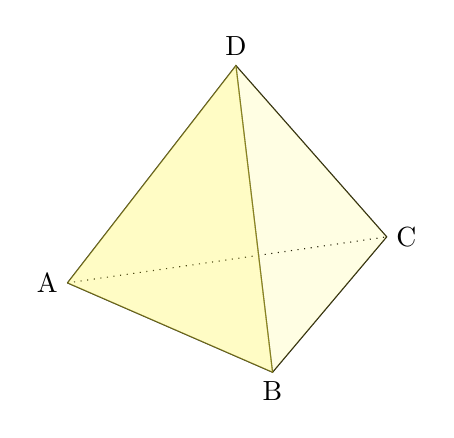
\begin{tikzpicture}[scale=0.5]
        \coordinate (A) at (0.95, 3.62);
        \coordinate (B) at (6.16, 1.35);
        \coordinate (C) at (9.06, 4.79);
        \coordinate (D) at (5.23, 9.14);
        \draw (A) -- (B) -- (C) -- (D) -- (A);
        \draw (B) -- (D);
        \draw [dotted] (A) -- (C);
        \filldraw [yellow!75,opacity=0.3] (A) -- (B) -- (D) -- cycle;
        \filldraw [yellow!75,opacity=0.15] (B) -- (C) -- (D) -- cycle;
        \node [left] at (A) {A};
        \node [below] at (B) {B};
        \node [right] at (C) {C};
        \node [above] at (D) {D};

    \end{tikzpicture}
\end{frame}

\begin{frame}{Exercício 9-5}
    \begin{itemize}
        \item Portanto, \(\vec{AB}\) e \(\vec{AD}\) são arestas de um triângulo equilátero:
    \begin{center}
        \begin{tikzpicture}[scale=2]
            \draw[thick] (0,0) coordinate[label=below:A] (A) --
                (1,0) coordinate[label=below:B] (B) --
                ($0.5*(1,0)+0.5*sqrt(3)*(0,1)$) coordinate[label=above:D] (C) --
                cycle;
            \draw[red] (0.15,0) arc (0:60:0.15);
            \node[red,right] at (0.1,0.15) {$60^\circ$};
        \end{tikzpicture}
    \end{center}
        \item Como a aresta é unitária, temos que
            \(\vec{AB}\cdot\vec{DA}=1 \cdot 1 \cdot \cos{\SI{120}{\degree}}=-1/2\)
    \end{itemize}
\end{frame}

\begin{frame}[c]{Exercício 9-7}
    São dados os números reais positivos \(a\) e \(b\), e o vetor \(\vec{u}\), de norma \(a\).
    Dentre os \(\vec{v}\) vetores de norma \(b\), qual é o que torna máximo o produto escalar \(\vec{u}\cdot\vec{v}\)?
    E mínimo? Quais são esses valores máximo e mínimo?
\end{frame}

\begin{frame}{Exercício 9-7}
    \begin{itemize}
        \item \(
            \vec{u}\cdot\vec{v}=||\vec{u}||\cdot ||\vec{v}||\cos{\theta}=
            ab\cos{\theta}
            \)
        \item Mas \(-1 \leq \cos{\theta} \leq 1\), onde \(
            \cos{\theta}=-1 \implies\theta=\SI{180}{\degree}\) e \(
            \cos{\theta}=1 \implies\theta=\SI{0}{\degree}\)
        \item \(\theta=\SI{0}{\degree} \implies \) vetores com mesmo sentido e direção
        \item \(\theta=\SI{180}{\degree} \implies \) vetores com mesma direção e sentidos opostos
        \item Assim, o vetor \(\vec{v}\) que dá o maior produto escalar é um vetor \textbf{paralelo} a \(\vec{u}\)
            % com módulo \(b\), ou seja,
            % \[
            %     \vec{v}=\frac{b}{a}\vec{u}
            % \]
            % de acordo com a definição de produto de um escalar por vetor
            e \( \vec{u}\cdot\vec{v}=ab\)

        \item Analogamente, o vetor \(\vec{v}\) que dá o menor produto escalar é um vetor \textbf{antiparalelo} a \(\vec{u}\)
            % com módulo \(b\), ou seja,
            % \[
            %     \vec{v}=-\frac{b}{a}\vec{u}
            % \]
            % de acordo com a definição de produto de um escalar por vetor
            e \( \vec{u}\cdot\vec{v}=-ab\)
    \end{itemize}

\end{frame}

\begin{frame}{Exercício 9-47}
    Prove que são verdadeiras as seguintes afirmações:
    \begin{itemize}
        \item \(\vec{AB}\cdot \vec{CD}+\vec{BC}\cdot\vec{AD}+\vec{CA}\cdot\vec{BD}=0\), quaisquer que sejam os pontos
            \(A\), \(B\), \(C\) e \(D\) (\textbf{Relação de Euler})
        \item Se um tetraedro tem dois pares de arestas opostas diagonais, as duas arestas restantes são
            ortogonais
        \item As três retas que contêm as alturas de um triângulo são concorrentes num ponto chamado \textit{ortocentro}
            do triângulo
    \end{itemize}

    \centering
    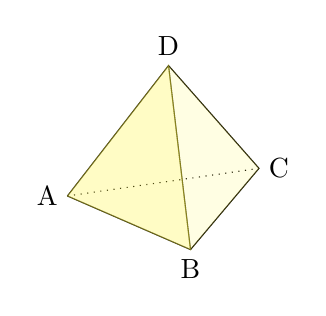
\begin{tikzpicture}[scale=0.3]
        \coordinate (A) at (0.95, 3.62);
        \coordinate (B) at (6.16, 1.35);
        \coordinate (C) at (9.06, 4.79);
        \coordinate (D) at (5.23, 9.14);
        \draw (A) -- (B) -- (C) -- (D) -- (A);
        \draw (B) -- (D);
        \draw [dotted] (A) -- (C);
        \filldraw [yellow!75,opacity=0.3] (A) -- (B) -- (D) -- cycle;
        \filldraw [yellow!75,opacity=0.15] (B) -- (C) -- (D) -- cycle;
        \node [left] at (A) {A};
        \node [below] at (B) {B};
        \node [right] at (C) {C};
        \node [above] at (D) {D};

    \end{tikzpicture}
\end{frame}

\begin{frame}{Exercício 9-50}
    Na Figura 9-3, a circunferência de centro \(O\) tem raio \(r\). Calcule \(\vec{BA}\cdot\vec{BC}\) em
    função de \(r\) e das medidas \(\alpha\) e \(\beta\) dos ângulos indicados. Aplique o resultado para
    provar que todo ângulo inscrito em uma semicircunferência é reto.

    \centering
    \begin{tikzpicture}[scale=1/3]
        \coordinate (A) at (0,0);
        \coordinate (O) at (8,0);
        \coordinate (B) at ($(O) + 8*({cos(60)},{sin(60)})$);
        \coordinate (C) at ($(O) + 8*({cos(30)},{-sin(30)})$);

        \draw [red] (O) circle (8);
        \draw [red] (A) -- +(16,0);
        \draw [red] (O) -- (B);
        \draw [red] (O) -- (C);
        \node [red, left] at (A) {A};
        \node [red,below] at (O) {O};
        \node [red, above right, shift={(-2pt,-2pt)}] at (B) {B};
        \node [red, below right, shift={(-2pt, 2pt)}] at (C) {C};
        \draw [red] (O) ++(3,0) arc (0:60:3) node [midway, shift={(3pt,3pt)}] {$\alpha$};
        \draw [red] (O) ++(3,0) arc (0:-30:3) node [midway, shift={(3pt,-2pt)}] {$\beta$};

    \end{tikzpicture}
\end{frame}

\begin{frame}{Estudo dirigido}
    \begin{itemize}
        \item Leia o assunto da Definição 9-12 e da Proposição 9-13 do livro texto (páginas 82 e 83)
        \item Resolva os exercícios 9-53 e 9-54, tirando dúvidas com o professor quando necessário
        \item Esses dois exercícios farão parte da lista da segunda prova
    \end{itemize}
\end{frame}

\begin{frame}{Exercício 9-36}
    A figura 9-5a mostra um paralelepípedo retângulo. Sendo \(\alpha\) e \(\beta\) as medidas
    dos ângulos indicados e \(\gamma\) a medida de \(A\hat{B}C\), mostre que \(\cos{\gamma}=\sen{\alpha}\sen{\beta}\)

    \centering
    \begin{tikzpicture}
        \coordinate (A) at (1.38,4.24);
        \coordinate (B) at (1.34,7.93);
        \coordinate (C) at (2.61,9.20);
        \coordinate (D) at (8.48,9.28);
        \coordinate (E) at (7.27,7.95);
        \coordinate (F) at (7.27,4.32);
        \coordinate (G) at (8.54,5.66);
        \coordinate (H) at (8.54,8.03);
        \coordinate (I) at (1.36,5.19);
        \coordinate (J) at (2.65,5.57);
        % \foreach \i in {A,..., J} {\node [red] at (\i) {\i};}

        \node [above] at (C) {B};
        \node [right] at (H) {C};
        \node [left] at (I) {A};

        \draw [blue] (A) -- (B) -- (C) -- (D) -- (G) -- (F) -- cycle;
        \draw [blue] (B) -- (E) -- (D);
        \draw [blue] (E) -- (F);
        \draw [blue, dotted] (A) -- (J) -- (C) (J) -- (G);
        \draw [blue, dotted] (C) -- (I);
        \draw [blue, dotted] (C) -- (H);

        \coordinate (P1) at ($(C)!0.2!(I)$);
        \coordinate (P2) at ($(C)!0.2!(H)$);
        \node [shift={(-2ex,-0.5ex)}] at (P1) {\small$\alpha$};
        \node [shift={(1.5ex,0.1ex)}] at (P2) {\small$\beta$};
        % \node [left, red] at (B) {J};
        % \node [right, red] at (D) {I};
        % \node [below right, xshift=-0.5ex, red] at (J) {K};
        \begin{scope}
            \clip (C) -- (D) -- (H);
            \filldraw [blue, opacity=0.1] let \p1=($(C)-(P2)$) in (C) circle ({veclen(\x1,\y1)});
        \end{scope}

        \begin{scope}
            \clip (C) -- (B) -- (I);
            \filldraw [blue, opacity=0.1] let \p1=($(C)-(P1)$) in (C) circle ({veclen(\x1,\y1)});
        \end{scope}
    \end{tikzpicture}
\end{frame}

